\chapter{Revisão Bibliográfica} \label{cap:rev}
Esse capitulo apresenta o embasamento teórico e trabalhos relacionados que juntos formam a base para o projeto proposto.

\section{Fundamentação teórica}
Essa sessão apresenta o embasamento teórico do trabalho proposto.

\subsection{Ensino de competências digitais para crianças}

Frequentemente são publicados novos estudos especulativos sobre as transformações que ocorrerão no mercado de trabalho no futuro. Apesar das análises e hipóteses variarem, a maioria aponta que diversas profissões de hoje ficarão obsoletas e em paralelo a isso, diversas outras novas profissões nascerão. No artigo \textit{21 Jobs Of The Future feito pela Cognizant Technology Solutions} \cite{cognizant_2017} vinte e uma novas profissões e suas principais habilidades são apontadas, servindo como um guia para conseguir um emprego ou se manter no mercado de trabalho nos próximos dez anos. Na maioria dessas novas profissões inferidas por esses e outros artigos, a habilidade de programar é aplicável direta e indiretamente. Algumas dessas profissões são: desenvolvedores de \textit{softwares}, engenheiros de \textit{machine learning}, analista de cibersegurança, engenheiros de \textit{big data}, cientista de dados, entre outras.

David Baker é um escritor, jornalista, fundador da TSOL Brasil, co-fundador da revista \textit{Wired} e um dos membros com mais antigos do corpo docente da \textit{The School of Life} de Londres. No ano de 2015 em uma palestra em São Paulo, Baker começa seu discurso com a seguinte afirmação: “O seu emprego pode não existir amanhã” \cite{carvalho_2015}. David Baker é bastante conhecido pelas suas pesquisas sobre as relação da tecnologia com o mercado de trabalho e afirma acreditar fortemente que logo grande parte das carreiras de hoje serão substituídas por robôs. Segundo Baker, não só carreiras braçais serão substituídas por robôs, mas “os engravatados também estão ameaçados”, brinca Baker.

Hoje, em 2020, já é possível ver essa migração. Indústrias de todos os tamanho, estão substituindo seus trabalhadores por robôs, um exemplo disso é a empresa de \textit{e-commerce} Amazon e sua logística interna, operada quase 100\% por tais máquinas \cite{winick_2018}. No mercado financeiro é possível observar Inteligências Artificiais atuando na compra e venda de ações de forma automatizada, com mais eficiência e assertividade do que analista financeiros. Na área da saúde, nano robôs já estão fazendo cirurgias. No setor de mobilidade urbana existem transportes completamente autônomos, como os caminhões sem motorista da empresa de transporte Uber que já transportam cargas sozinhos em rodovias americanas \cite{demartini_2016}. Até mesmo em trabalhos que exigem habilidades criativas, podemos ver robôs atuando e um exemplo disso é o comercial de uma marca de veículos de luxo escrito totalmente por uma inteligência artificial \cite{autran_2018}.

Sendo assim, torna-se evidente a importância de preparar as crianças de hoje para o mercado de trabalho do futuro. Para tal desenvolvimento, uma das habilidades mais importantes é a programação. Um exemplo dessa relevância foi a recente atualização da Base Nacional Comum Curricular (BNCC) realizada pelo Ministério da Educação (MEC). Nessa atualização, a BNCC dedica uma de suas dez competências para as tecnologias digitais no seu conceito de educação integral. Segundo a BNCC:

\begin{citacao}

Compreender, utilizar e criar tecnologias digitais de informação e comunicação de forma crítica, significativa, reflexiva e ética nas diversas práticas sociais (incluindo as escolares) para se comunicar, acessar e disseminar informações, produzir conhecimentos, resolver problemas e exercer protagonismo e autoria na vida pessoal e coletiva \cite[p. 9]{bncc_2017}.

\end{citacao}

Analisando esse trecho da Base Nacional Comum Curricular, é possível reconhecer argumentos em prol da inserção de programação na Educação Básica, como ao apontar que tecnologias digitais podem ser um excelente recurso para a comunicação de informações e resolução de problemas. A BNCC também menciona o termo “pensamento computacional” no Caderno de Matemática, comentando a importância de fluxogramas e algoritmos, que podem ser estudados nas aulas de Matemática \cite{bncc_2017}.

Em um estudo sobre ensino inicial de Programação e Robótica Educacional \cite{antonello_cardoso_2015} é apontado que o ensino de programação pode ser interdisciplinar, ou seja, pode abranger duas ou mais áreas de conhecimento. O ensino de programação pode proporcionar interação e progresso em duas disciplinas ao mesmo tempo, desenvolvendo \textit{hard skills}, entendidas como competências técnicas. Do mesmo modo, esse ensino está diretamente ligado ao desenvolvimento de \textit{soft skills}, que são habilidades que trabalham com a relação dos indivíduos com os outros e com eles mesmos. Essas são competências como: resiliência, colaboração e comunicação, afirma o autor do livro best seller “Inteligência Emocional” \cite{goleman_2012}.

O artigo “Programar é bom para as crianças? Uma visão crítica sobre o ensino de programação nas escolas” \cite{geraldes_2014} mostra — por meio do Scratch, que é uma ferramenta de ensino de programação em blocos para crianças — que o ensino da programação desenvolve competências como criatividade e raciocínio lógico, além de estimular o aprendizado de inglês, trabalho em equipe, resolução de problemas, entre outras.

Mesmo com todos esses benefícios, ainda é pequeno o número de professores que fazem realmente o uso de tecnologias ou ensinam programação e outras tecnologias em sala de aula, os que usam, fazem somente uso de laboratórios de informática, como diz o estudo do Programa Nacional de Formação Continuada em Tecnologia Educacional \cite{suenia_andre_2012}. Esse estudo mostra que professores têm insegurança ao utilizar tecnologias em sala de aula, observa-se retratado no mesmo estudo que a inserção de novas tecnologias nas escolas sofre de falta de investimentos também. Portanto, nota-se que há uma carência de tecnologias que sejam acessíveis financeiramente e que os professores possam utilizá-las facilmente e intuitivamente em sala de aula. Também existem necessidades por parte dos alunos.

Em um artigo apresentado no Congresso Internacional de Educação e Tecnologias \cite{lima_queiroz_santana_2018}, são apresentados os seguintes estilos de aprendizagem: visual, auditivo e cinestésico. Assim, também é retratada a dificuldade do aluno de hoje em se concentrar em aulas realizadas com os métodos tradicionais e antiquados. Esse estudo ressalta a importância do uso de TIDCs (Tecnologias Digitais de Informação e Comunicação) em sala de aula, pois, segundo o estudo, TIDCs conseguem alinhar os estilos de aprendizado além de aumentar a concentração e motivação dos alunos. É por esse motivo, que na sala de aula se faz necessário observar a dinâmica do dia a dia, assim como as particularidades dos alunos, como idade, região em que vivem, interesses, etc. De acordo com o professor húngaro \cite[p. 81]{dornyei_2001} existem algumas estratégias motivacionais que demonstram efetividade no ensino, são elas: o aumento da interação dos alunos, a atribuição de tarefas interessantes e a quebra da monotonia da aprendizagem. Logo, se trabalhadas de forma interligada, essas estratégias podem tornar as aulas mais instigantes e estimular o desejo de aprender nos alunos.

Ademais, habilidades tecnológicas se tornam cada vez mais requisitadas no mercado de trabalho, reforçando assim a importância do contato do aluno com esses conceitos e ferramentas. Tendo em vista essa dificuldade de concentração dos alunos, é necessário criar estratégias que estimulem o aprendizado dos alunos. \citeonline{jacobsen_maffei_sperotto_2013}, sugerem o uso de jogos eletrônicos, pois por serem lúdicos, os jogos tornam a aprendizagem mais eficiente. Já que estimulam o raciocínio rápido, auxiliam na assimilação de conceitos complexos e desenvolvem a criatividade, isso porque com jogos os alunos deixam de ser ouvintes e passam a ser protagonistas do seu aprendizado. Nesse mesmo artigo, “Jogos eletrônicos: um artefato tecnológico para o ensino e para a aprendizagem”, nota-se que jogos não auxiliam apenas no aprendizado do conteúdo abordado em um determinado jogo, mas estimulam o desenvolvimento de outras competências como convivência, cooperação, troca de ideias, cumprimento de regras, entre outros hábitos de interação. Assim, acredita-se que a inserção de jogos eletrônicos pode funcionar como motivação para os alunos.

\subsection{Ensino da sustentabilidade}

Outro ponto considerado importante no âmbito da educação é o ensino da sustentabilidade. No ano de 2016, cerca de 40\% dos resíduos sólidos não foram destinados corretamente, ou seja, por volta de 30 milhões de toneladas \cite{abrelpe_2017}. Pode-se afirmar que tal ação não é benéfica para o meio ambiente, já que esse material pode acabar em rios, gerar enchentes e causar impactos na saúde pública. Da totalidade de lixo produzido em território brasileiro, cerca de 30\% poderia ser reciclado, entretanto somente 3\% disso é realmente reciclado \cite{pnrs_2010}. Um dos principais motivos disso é o fato do lixo orgânico e reciclável não serem descartados corretamente. Desse modo, reciclar é uma ótima alternativa para amenizar a problemática de resíduos urbanos, impactando diretamente o meio ambiente, sociedade e economia.

De acordo com a “Agenda 2030 para o Desenvolvimento Sustentável”, a ONU (Organizações das Nações Unidas) tem como objetivo reduzir consideravelmente os resíduos até o ano de 2030 \cite{onu30_2015}. A ideia é fazer isso por meio prevenção, da reciclagem e do reuso. Tal ação pode ser desenvolvida por meio da Educação Ambiental. Essa estratégia possibilita a sensibilização dos alunos em relação ao meio ambiente, instruindo-os a refletir sobre a poluição e os danos causados à natureza. Sobre esse tema os PCNS (Parâmetros
Curriculares Nacionais) apontam que:

\begin{citacao}

    O trabalho com o tema Meio Ambiente deve ser desenvolvido visando-se proporcionar aos alunos uma diversidade de experiências e ensinar-lhes formas de participação, para que possam ampliar a consciência sobre as questões relativas ao meio ambiente e assumirem de forma independente e autônoma atitudes e valores voltados à sua proteção e melhoria \cite[p. 46]{pcns_2001}.

\end{citacao}

Sendo assim, ao desenvolver esse tema no ambiente escolar, pode-se ensinar aos estudantes o respeito à natureza e o cuidado com o meio ambiente. Um bom jeito de trabalhar esse tema é por meio da reciclagem, ensinando as crianças sobre os benefícios que esse ato pode trazer para o meio ambiente e para eles mesmos.

Por fim, considerando os conceitos apresentados previamente é possível julgar como relevante trabalhar com o uso de programação e de jogos nas escolas. Já que essas têm capacidade de abranger diversas áreas do conhecimento, além de poder desenvolver habilidades emocionais. Assim, esse projeto visa unir o ensino de programação por meio de jogos com o tema de reciclagem, a fim de criar uma excelente ferramenta para o ensino dessas áreas nas escolas.

\subsection{Unity como ferramenta de criação de Jogos}

O Unity foi criado em 2005 por David Helgason, Joachim Ante e Nicholas
Francis na Dinamarca. É uma ferramenta com bastante força no mercado de jogos por suportar o desenvolvimento para diversas plataformas digitais. 50\% dos jogos entre todas as plataformas são feitos usando Unity tendo mais de 3 bilhões de dispositivos alcançados no mundo todo \cite{dados_unity}.

Muitos jogos criados no Unity alcançaram sucesso de vendas e se tornaram bastante conhecidos, por exemplo o jogo Cuphead, criado pelo StudioMDHR lançado em 2017 para as plataformas Xbox One, Windows 10, e Steam \cite{cuphead}. Outro jogo bastante conhecido é o Monument Valley 2 lançado em 2017 para as plataformas Android e IOS\cite{monument_valley_2}.


\section{Trabalhos Relacionados}
Esse tópico apresentará os trabalhos relacionados ao projeto proposto.

\subsection{Academia}
Após refletir sobre a importância do ensino de programação para crianças, principalmente por meio de jogos digitais, pode-se observar diversas pesquisas sendo realizadas para testar e validar novas abordagens e aplicações. 

Observa-se no trabalho “Jogos Digitais no Ensino de Conceitos de Programação para Crianças” \cite{tadesco_2016}, o qual faz uso de jogos digitais gratuitos com foco em ensino de programação como por exemplo o \textit{Code Monkey}, representado na Figura \ref{figura:code_monkey}, que o uso dessa tecnologia beneficia a apresentação de conteúdo além de manter os alunos engajados durante a aula. Os testes neste trabalho foram realizados com alunos entre cinco e seis anos de uma escola privada em algumas aulas no primeiro semestre letivo no ano de 2016. Após de algumas sessões, os alunos foram desafiados a resolver alguns níveis mais complexo em um determinado jogo para comprovar a efetividade do estudo. Nas primeiras análise, fica claro que o uso dessa metodologia é  interessante para o ensino de lógica de programação nessa faixa etária, pois maioria dos alunos conseguiu passar pela maioria dos desafios, e apenas poucos alunos demonstraram dificuldade em aplicar os conceitos de laços de repetição. Segundo os autores, alguns elementos das interfaces gráfica dos jogos escolhidos deveriam ser aperfeiçoadas pensando na faixa etária dos alunos.

\begin{figure}[H]
    \caption{Jogo Code Monkey}
    \centering
        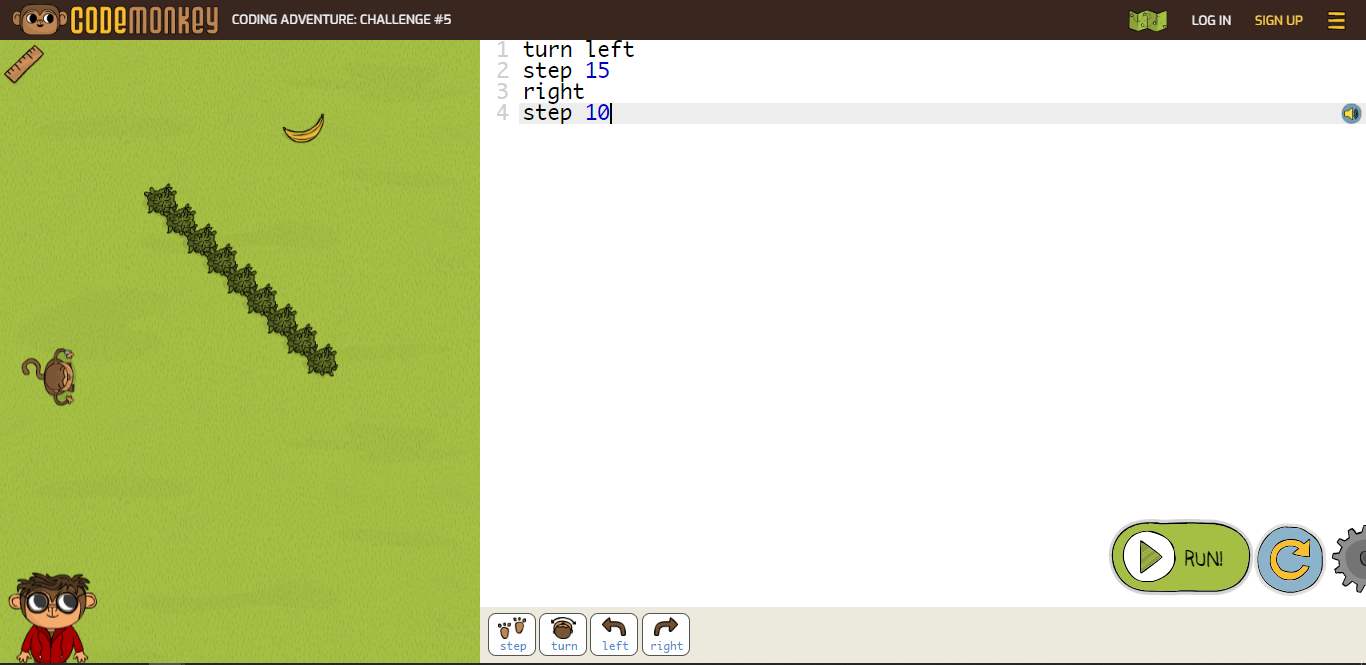
\includegraphics[width=\linewidth]{Imagens/cap2/code_monkey.png}
    \legend{\small{Fonte: \citeonline{code_monkey}}}
    \label{figura:code_monkey}
\end{figure}

Além de testes com ferramentas já conhecidas, podemos ver também na academia o desenvolvimento de novas soluções utilizando jogos digitais para trabalhar outros conceitos ou o próprio conceito da programação. No artigo \textit{"Towards a Tangible User Interface Embedded Computing Prototype For Child Education"} \cite{carneiro_2018}, foram desenvolvidos três jogos digitais com o objetivo de trabalhar e exercitar conceitos básicos de matemática para crianças que estão iniciando a alfabetização matemática. Além dos jogos, foi desenvolvido também uma base física que comportava seis blocos e os blocos numéricos individuais, ou seja, cada bloco com um número. Neste trabalho, os jogos propostos eram jogados por meio dessa estrutura física, como demonstrado na Figura \ref{figura:estrutura_artigo_towards}, para promover uma maior interação da criança com os jogos. Portanto, era proposto então um desafio matemático para a criança e após a resolução desse desafio, a criança deveria colocar na base os cubos numéricos com a resolução do desafio e apertar um botão para enviar sua resposta, para por fim receber uma mensagem de “correto” ou “incorreto”. Não houveram testes para comprovar a efetividade da solução. 

\begin{figure}[H]
    \caption{Estrutura Fisica do artigo \textit{"Towards a tangible user interface embedded computing prototype for child education”}}
    \centering
        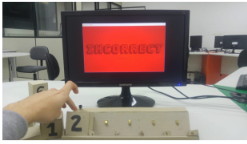
\includegraphics[width=\linewidth]{Imagens/cap2/estrutura_artigo_towards.png}
    \legend{\small{Fonte: \cite{carneiro_2018}}}
    \label{figura:estrutura_artigo_towards}
\end{figure}

Pode-se utilizar de jogos digitais para facilitar ou até mesmo possibilitar o ensino de disciplinas tradicionais na grade curricular brasileira, como por exemplo no artigo “Jogos Digitais No Ensino Da Língua Portuguesa Para Crianças Surdas” \cite{liz_2017} que utilizou jogos digitais para ensinar a língua portuguesa e em um contexto de acessibilidade. Neste artigo os pesquisadores relatam o projeto de Educomunicação feito pela Universidade Estadual de Campinas em parceria com uma escola municipal do estado de São Paulo. O objetivo foi desenvolver jogos digitais para tablets para possibilitar o ensino da língua portuguesa como língua secundária para alunos com deficiência auditiva de primeiro a quinto ano, em uma turma bilíngue. O método de validação, foi uma análise comparativa de desempenho baseado em duas atividades: uma das atividades continha palavras que foram trabalhadas nos jogos digitais e a segunda atividade continha palavras que não foram trabalhadas por meio desse recurso. Por meio da avaliação comparativa, pode-se ver que houveram mais respostas certas nas atividades com palavras que receberam intervenção dos jogos digitais desenvolvidos pelas pesquisadoras. Por fim, por meio dos testes, a  pesquisa pôde concluir que, jogos digitais são uma estratégia importante para o ensino da língua portuguesa para crianças com deficiência auditiva.

\subsection{Mercado}
Assim como no meio acadêmico, pode-se ver no mercado um movimento para o desenvolvimento de novas soluções digitais com foco na educação também. 
No ano de 2007, o \textit{Media Lab} do \textit{Massachusetts Institute of Technology} (MIT) desenvolveu uma linguagem de programação em blocos com o objetivo de ensinar crianças o pensamento criativo, trabalho colaborativo e pensamento sistemático, habilidades essenciais para o século XXI \cite{about_scratch}. Hoje, além de um ferramenta de programação, o Scratch é também uma comunidade online na qual crianças podem programar jogos, histórias e animações e compartilhar essas criações com o mundo, como pode-se ver na Figura \ref{figura:scratch}. O Scratch foi desenvolvido principalmente para crianças entre oito e dezesseis anos, mas segundo a própria ferramenta, é usado por milhões de pessoas de todas as idades. Hoje o scratch se encontra em casas e escolas de mais de cento e cinquenta países e é usado para trabalhar diversas disciplinas como matemática, ciência da computação, linguagens, artes, entre outras. Por conta de seu alcance, o Scratch está disponível em mais de quarenta línguas. Em 2016 a Scratch Foundation tornou pública uma parceria com a gigante Google para uma atualização da ferramenta, e o lançamento da versão 3.0 do Scratch ocorreu em janeiro de 2019.

\begin{figure}[H]
    \caption{Plataforma Scratch}
    \centering
        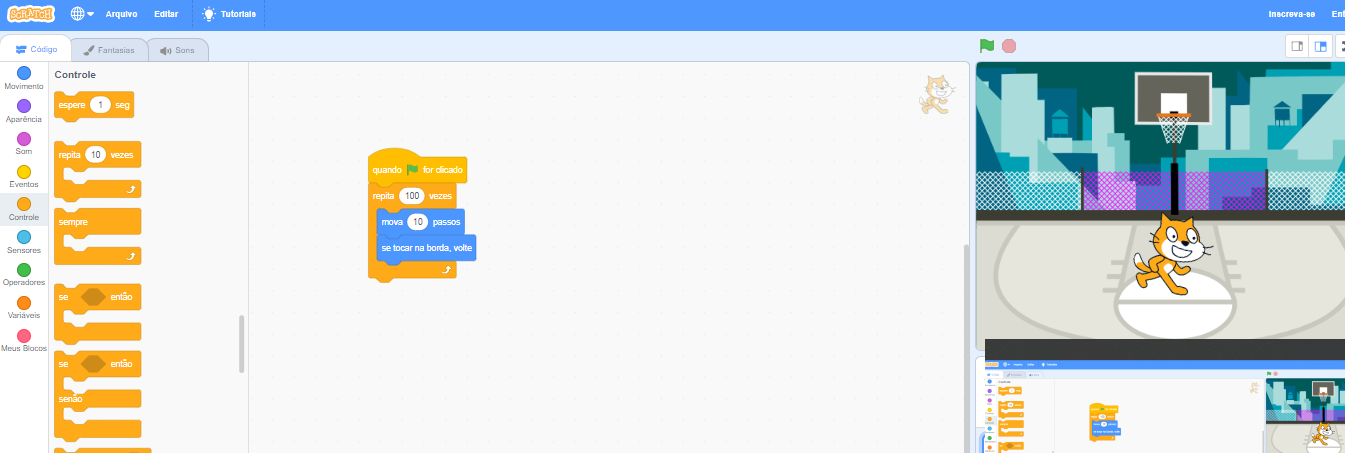
\includegraphics[width=\linewidth]{Imagens/cap2/scratch.png}
    \legend{\small{Fonte: \citeonline{about_scratch}}}
    \label{figura:scratch}
\end{figure}

Em 2015, a emissora britânica British Broadcasting Corporation (BBC), fez o anúncio da iniciativa Make it Digital com o objetivo de “inspirar os visionários digitais do futuro” como diz seu Diretor Geral Tony Hall. Parte dos esforços dessa iniciativa era o desenvolvimento de um microcomputador barato, portátil e fácil de programar, o que deu origem ao BBC micro:bit. O BBC micro:bit é uma placa de circuitos elétricos, tem um conector Universal Serial Bus (USB) para alimentação e transferência de dados, e, o que mais chama atenção na placa, é sua gama diversa de sensores como botões, termômetro, luxímetro, magnetrônomo e acelerômetro. Além disso, a placa conta com vinte e cinco leds vermelhos dispostos em uma matriz cinco por cinco e possui também contatos para conexão de periféricos externos. O objetivo da placa com todas essas possibilidades é, fazer com que as crianças tenham mais interesse por eletrônica e programação. Pensando na demanda das escolas de preparar profissionais com habilidades tecnológicas e, juntamente com as novas diretrizes da BNCC, a empresa brasileira Tecnologia Educacional com a solução Inventura, já colocou o BBC micro:bit em diversas escolas brasileiras em um material que, além de trabalhar competências técnicas, trabalha também competências como comunicação, colaboração, pensamento analítico, curiosidade, imaginação, entre outros \cite{about_microbit}. 

Segundo o World Economic Forum, sessenta e cinco por cento das crianças que estão entrando na escola primária hoje, terão trabalhos que ainda não existem. Pensando  nesses dados e observando toda essa mudança acontecendo no meio educacional, a empresa dinamarquesa de blocos de montar, LEGO, desenvolveu diversos produtos que permeiam esse contexto. Um dos mais famosos é o LEGO\textsuperscript{®} MINDSTORMS \textsuperscript{®} Education EV3, pensado para alunos do ensino médio e fundamental II. O Education EV3 é um produto de robótica educacional que incentiva o ensino STEAM (Science, Technology, Engineering, Art and Math). Além dos blocos de montar normais que são comuns nos produtos da empresa, o produto conta com o bloco EV3, que é um computador programável capaz de receber informação de sensores e controlar atuadores. O EV3 é programável através um software da mesma empresa disponível para tablets e computadores \cite{lego_mindstorms}. O software LabVIEW é um ambiente de programação gráfico que faz uso de blocos para estruturar comando para o EV3, como mostrado Figura \ref{figura:labview}, tornando a programação simples e intuitiva. 

\begin{figure}[H]
    \caption{Interface LabVIEW}
    \centering
        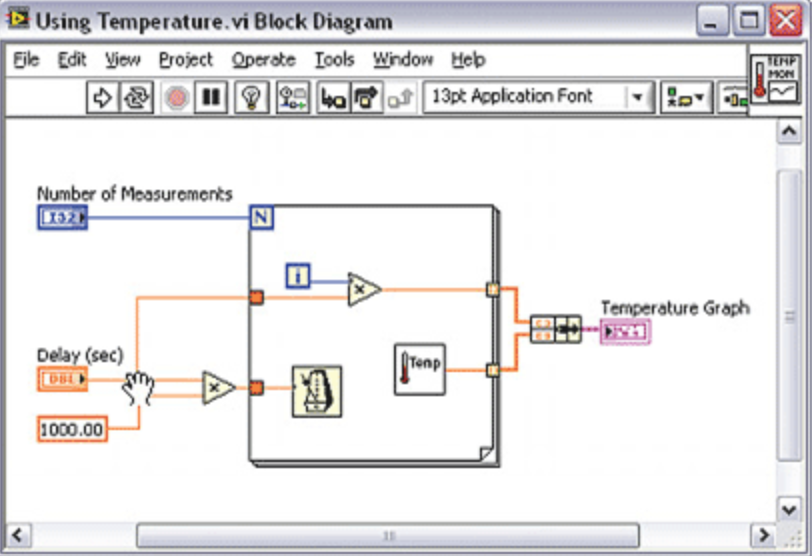
\includegraphics[width=\linewidth]{Imagens/cap2/labview.png}
    \legend{\small{Fonte: \cite{labview}}}
    \label{figura:labview}
\end{figure}

\subsection{Comentários}
Observa-se diversos esforços da academia e do mercado para desenvolver pesquisas, produtos e novas soluções para preparar as crianças que estão entrando agora no ensino básico para assumir futuros novos empregos. Esses esforços também focam em motivar e aprimorar o ensino dessas crianças por meio de novas estratégias educacionais, como  por exemplo jogos digitais. Pensando nisso, o trabalho proposto tem como objetivo ensinar programação por meio de jogos digitais como no artigo “Jogos Digitais no Ensino de Conceitos de Programação para Criança" \cite{tadesco_2016} que mostra as vantagens dessa metodologia para o ensino de programação para crianças. Fica claro por meio do artigo "Jogos Digitais No Ensino Da Língua Portuguesa Para Crianças Surdas" \cite{liz_2017} o potencial de jogos digitais para o ensino de diversas disciplinas, portanto este trabalho abordará o tema da reciclagem como cenário do jogo proposto com o objetivo de, além de programação, ensinar também sobre sustentabilidade. Considerando a importância de recursos que aumentam a interatividade das crianças com o ensino como visto no artigo \textit{"Towards a Tangible User Interface Embedded Computing Prototype For Child Education"} \cite{carneiro_2018}, o trabalho proposto, além do uso de jogos digitais, também fará uso de blocos físicos para promover uma maior interatividade com a criança tornando-a assim ainda mais protagonista do seu aprendizado. A escolha do uso dos blocos para o ensino da programação se deu por conta da comprovação de sua efetividade considerando a sua ampla utilização no mercado em soluções como o Scratch e do EV3 da Lego education, pois torna programação mais simples, interativa e intuitiva. 




